% [Overleaf] https://www.overleaf.com/read/nbnhdyqmdqyz
% [YouTube] https://youtu.be/VU0ksglb7Rw
% [GitHub] https://github.com/nobucshirai/infona2020_slide_12
\documentclass[dvipdfmx,aspectratio=169,20pt]{beamer}
\usepackage{bxdpx-beamer}

% Beamer theme
\usetheme{Boadilla}

%%%%% JAPANESE FONT SETTINGS %%%%%
\usepackage[utf8]{inputenc}
\usepackage{pxjahyper}
\renewcommand{\kanjifamilydefault}{\gtdefault} % for Gothic Japanese fonts
\newcommand{\myfontsetting}[3]{{\fontsize{#1}{#2}\selectfont #3}}
\usepackage[deluxe,uplatex]{otf} % needed to use super bold Japanese fonts
\usepackage[unicode,noto-otc]{pxchfon} % needed to use super bold Japanese fonts
%%%%%%%%%%%%%%%%%%%%%%%%%%%%%%%%%%

%%%%% SETTINGS FOR MATH SYMBOLS %%%%%
\usepackage{amsmath,amssymb}
\usepackage{bm}
%\usepackage{graphicx}
\usepackage{latexsym}
\usefonttheme{professionalfonts} % use Serif fonts for equations
%%%%%%%%%%%%%%%%%%%%%%%%%%%%%%%%%%%%%

\usepackage{fancybox,ascmac}
\usepackage{url}
\usepackage[many]{tcolorbox}

%%%%% ALGORITHM SETTING %%%%%
\usepackage{algorithm}
\usepackage[noend]{algorithmic}
\algsetup{linenosize=\color{fg!50}\fontsize{8pt}{8pt}\selectfont}
\renewcommand\algorithmicdo{\bfseries :}
\renewcommand\algorithmicthen{\bfseries :}
\renewcommand\algorithmicrequire{\textbf{Input:}}
\renewcommand\algorithmicensure{\textbf{Output:}}
\renewcommand{\algorithmicprint}{\textbf{break}}
%%%%%%%%%%%%%%%%%%%%%%%%%%%%%
\definecolor{myblue1}{RGB}{45,130,200}
\definecolor{myblue2}{RGB}{26,89,142}
\setbeamertemplate{navigation symbols}{}
\setbeamercolor*{structure}{fg=myblue1,bg=blue}
\setbeamercolor{block title}{fg=myblue1!50!black}
\setbeamercolor*{block title example}{fg=white,bg=myblue2}
\setbeamercolor*{palette primary}{use=structure,fg=white,bg=structure.fg}
\setbeamercolor*{palette secondary}{use=structure,fg=white,bg=structure.fg!75!black}
\setbeamercolor*{palette tertiary}{use=structure,fg=white,bg=structure.fg!50!black}
\setbeamercolor*{palette quaternary}{fg=black,bg=myblue1}

\setbeamerfont{alerted text}{series=\bfseries}
\setbeamerfont{section in toc}{series=\mdseries}
\setbeamerfont{frametitle}{size=\Large,series=\bfseries}
\setbeamerfont{title}{size=\LARGE,series=\bfseries}
\setbeamerfont{date}{size=\small}

\setbeamertemplate{block title}[shadow=false]
\setbeamertemplate{blocks}[rounded][shadow=false]

%%%%% BEAMER FOOTLINE SETTINGS %%%%%%
\setbeamertemplate{footline}[frame number]{}
\setbeamerfont{footline}{size=\bf\footnotesize\small}
%%%%%%%%%%%%%%%%%%%%%%%%%%%%%%%%%%%%%

%%%%% BEAMER ITEM SETTINGS %%%%%
\setbeamertemplate{itemize item}[circle]
\setbeamertemplate{itemize subitem}[triangle]
\setbeamertemplate{enumerate item}[circle]
%%%%%%%%%%%%%%%%%%%%%%%%%%%%%%%%

\begin{document}

%%%%%%%%%%%%%%%%%%%%%%%%%%%%%%%%
\begin{frame}
%%%%% START_TAG B %%%%%
%\noindent{\bf X\hspace{-.1em}I-B.}
\frametitle{[問題] X\hspace{-.1em}I-B}

\myfontsetting{18pt}{18pt}{
X\hspace{-.1em}I-A で示した定積分をシンプソン則を用いて数値積分する問題を考える。ニュートン・コーツ則で2次多項式近似を行う区間の数を $M=2^{n-1}$ (積分点間の区画の数は $2M=2^n$、積分点の数は $2M+1=2^n+1$) とした時の $n\ge 1$ を1ずつ増やして積分値を求めるプログラムを作成し、数値積分の値の相対誤差が $10^{-8}$ を下回る最も小さい $n$ を求めよ。
}\\
\myfontsetting{12pt}{12pt}{
作成したプログラムも提出すること。プログラミング言語は問わない。
}
%%%%% END_TAG B %%%%%
\end{frame}
%%%%%%%%%%%%%%%%%%%%%%%%%%%%%%%%
\begin{frame}
\frametitle{[略解] X\hspace{-.1em}I-B}

$n=5$ $(M=16)$

\end{frame}
%%%%%%%%%%%%%%%%%%%%%%%%%%%%%%%%
%タイトルページ

\title{\myfontsetting{32pt}{32pt}{常微分方程式の数値解法 (1)}}

\titlegraphic{\vspace{-7mm}\flushright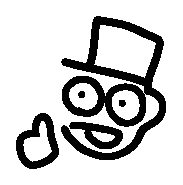
\includegraphics[width=1.8cm,height=1.8cm]{hattari_kun_good_org.eps}}

\setbeamertemplate{title page}{%
    \begin{flushright}
        \usebeamercolor[fg]{titlegraphic}\inserttitlegraphic
    \end{flushright}
    \vspace{-0.6cm}
    \hspace{1.5cm}{\selectfont\usebeamerfont{subtitle} \usebeamercolor[fg]{subtitle} [\href{https://youtu.be/VU0ksglb7Rw}{数値解析 第12回}] \par}
    \vspace{0.5cm}
    %\vspace{2.5em}
    {\centering\usebeamerfont{title} \usebeamercolor[fg]{title} \inserttitle \par}
    \vspace{0.5cm}
    \begin{center}
        近似を重ねて少しずつ伸ばす
    \end{center}
}

\date[\todey]{}

\frame{\titlepage}

%%%%%%%%%%%%%%%%%%%%%%%%%%%%%%%%
\begin{frame}
\frametitle{\myfontsetting{24pt}{24pt}{常微分方程式の問題設定}}
\begin{block}{{\bf\small 常微分方程式} {\small (Ordinary differential equation, ODE)}}
\myfontsetting{14pt}{14pt}{
1変数関数 $y(t)$ の導関数を含む方程式を{\bf 常微分方程式}と呼ぶ。$y(t)$ の導関数の最高次が $n$ の時 {\bf n階常微分方程式}と呼ぶ。
常微分方程式の解法では方程式を満たす関数 $y(t)$ を求める。
}
\end{block}

\vspace{-3mm}

\begin{itemize}
    %\setlength{\itemsep}{0.5cm}
    \item \myfontsetting{13pt}{13pt}{1階常微分方程式は $\frac{dy(t)}{dt}=f(t,y(t))$ の形に書ける}
    \item 
    \myfontsetting{13pt}{13pt}{n階常微分方程式は $n+1$ 変数$n$ 本の1階常微分方程式に分解できる}
    %\item  \myfontsetting{14pt}{16pt}{常微分方程式の数値解法}
    \begin{itemize}
        \item \myfontsetting{10pt}{12pt}{n階常微分方程式 $\frac{d^n y}{dt^n} = f\left(t,y,\frac{dy}{dt}, \dots, \frac{d^{n-1} y}{dt^{n-1}}\right)$ に対して
        $y_1=y$, $y_2=\frac{dy_1}{dt}$,$\dots$, $y_{n+1}=\frac{d y_n}{dt}$ と置くと $\frac{dy_i}{dt} = f_i(t, y_1, y_2, \dots, y_{n+1})$ \myfontsetting{8pt}{8pt}{$(1\le i \le n)$} のように書き換えられる $\to$ \myfontsetting{8pt}{8pt}{\bf 1階常微分方程式が解けたらn階常微分方程式も (原理的には) 解ける}}
    \end{itemize}
\end{itemize}
\end{frame}
%%%%%%%%%%%%%%%%%%%%%%%%%%%%%%%%
\begin{frame}
\frametitle{\myfontsetting{24pt}{24pt}{勾配場を用いた1階微分方程式の図解}}
\begin{columns}[t]
\begin{column}{0.48\textwidth} 
\vspace{-7mm}
\begin{itemize}
    \setlength{\itemsep}{0.25cm}
    \item 
    \myfontsetting{15pt}{17pt}{
    1階微分方程式 $\frac{dy}{dt}=f(t,y)$ の右辺を{\bf 勾配場} (Slope field) と呼ばれる $t$--$y$ 平面上の図にすると理解が深まる
    }
    \begin{itemize}
        \item 
        \myfontsetting{10pt}{10pt}{
        勾配場では $t$--$y$ 平面上に $f(t,y)$ の値を棒の傾きで表示する
        ($\tan \theta = f(t,y)$)
        }
    \end{itemize}
\end{itemize}
\end{column}
\begin{column}{0.52\textwidth} 
\begin{figure}[h]
	\begin{center}
\vspace{-10mm}
    	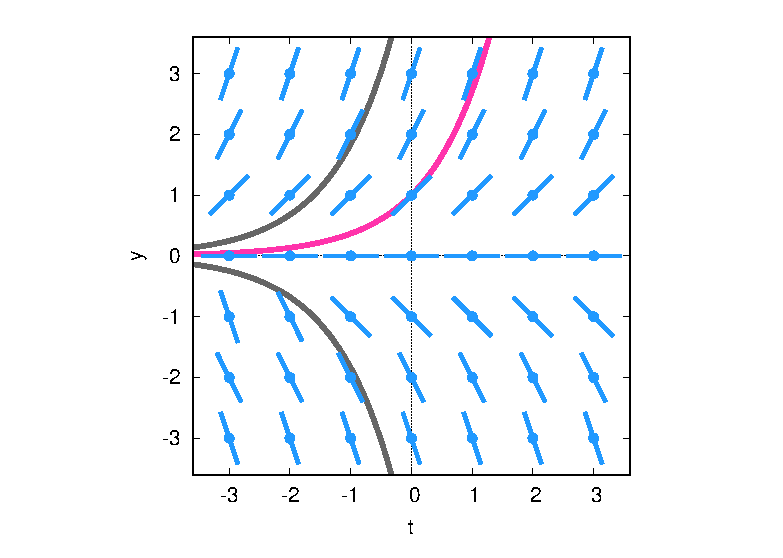
\includegraphics[width=1.0\textwidth]{fig12-1_differential_equation_example.eps}
	\end{center}
	\vspace{-5mm}
	\caption{\myfontsetting{10pt}{10pt}{$f(t,y)$ の大きさを棒の傾きで表現した勾配場}}
\end{figure}
\end{column}
\end{columns}
\end{frame}
%%%%%%%%%%%%%%%%%%%%%%%%%%%%%%%%
\begin{frame}
\frametitle{\myfontsetting{28pt}{28pt}{[図解] $f(t,y) = 1$ の勾配場}}
\begin{columns}[t]
\begin{column}{0.48\textwidth} 
\vspace{-8mm}
\begin{itemize}
    %\setlength{\itemsep}{0.25cm}
    \item 
    \myfontsetting{12pt}{12pt}{
    $\frac{dy}{dt} = 1$ の一般解は $y=t+C$ \myfontsetting{10pt}{10pt}{($C$ は積分定数)}
    }
    \vspace{-1mm}
    \item 
    \myfontsetting{12pt}{12pt}{
    $f(t,y)$ の図は $t$--$y$ 平面に傾き1の棒を敷き詰めたものになる
    }
    \vspace{-1mm}
    \item \myfontsetting{12pt}{12pt}{
        初期点 $(t,y)$ をどこに置くかで縦方向にずれたどの直線に乗るかが決まる
        \myfontsetting{10pt}{10pt}{(これは積分定数の不定性に対応する)}
        }
\end{itemize}
\end{column}

\begin{column}{0.52\textwidth} 
\begin{figure}[h]
	\begin{center}
\vspace{-10mm}
    	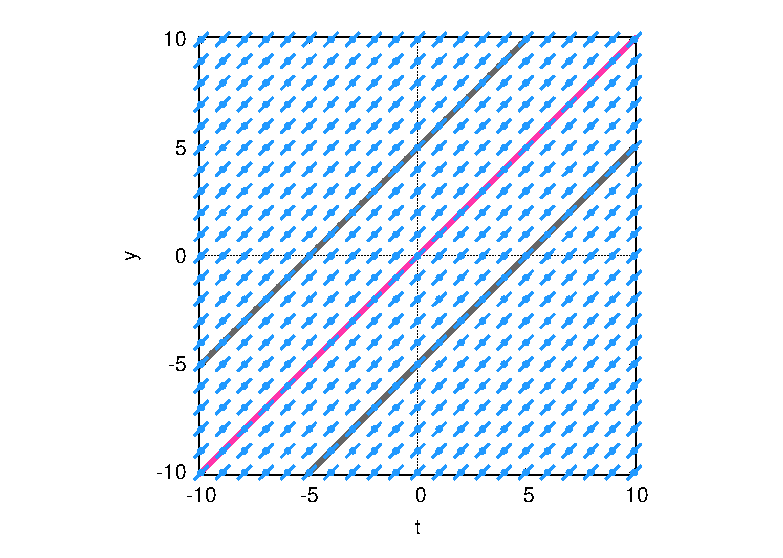
\includegraphics[width=1.0\textwidth]{fig12-2_differential_equation_const.eps}
	\end{center}
	\vspace{-5mm}
	\caption{\myfontsetting{10pt}{10pt}{$f(t,y)=1$ を図示したもの。$y=t+C$ が見て取れる。}}
\end{figure}
\end{column}
\end{columns}
\end{frame}
%%%%%%%%%%%%%%%%%%%%%%%%%%%%%%%%
\begin{frame}
\frametitle{\myfontsetting{28pt}{28pt}{[図解] $f(t,y) = t$ の勾配場}}
\begin{columns}[t]
\begin{column}{0.48\textwidth} 
\vspace{-8mm}
\begin{itemize}
    %\setlength{\itemsep}{0.25cm}
    \item 
    \myfontsetting{12pt}{12pt}{
    $\frac{dy}{dt} = t$ の一般解は $y=\frac{1}{2}t^2+C$ \myfontsetting{10pt}{10pt}{($C$ は積分定数)}
    }
    \vspace{-1mm}
    \item 
    \myfontsetting{12pt}{12pt}{
    棒の傾きは $y$ 軸方向には変化せず $t$ 軸方向にのみ変化する
    }\\
    \vspace{-2mm}
    \myfontsetting{6pt}{6pt}{
    ($t=0$ で傾き0、 $t>0$ で正の傾き、 $t<0$ で負の傾き)
    }
    \vspace{-1mm}
    \item \myfontsetting{12pt}{12pt}{
        初期点の置き方によって縦方向にずれたどの放物線に乗るかが決まる
        \myfontsetting{10pt}{10pt}{(積分定数の不定性に対応)}
        }
\end{itemize}
\end{column}

\begin{column}{0.52\textwidth} 
\begin{figure}[h]
	\begin{center}
\vspace{-10mm}
    	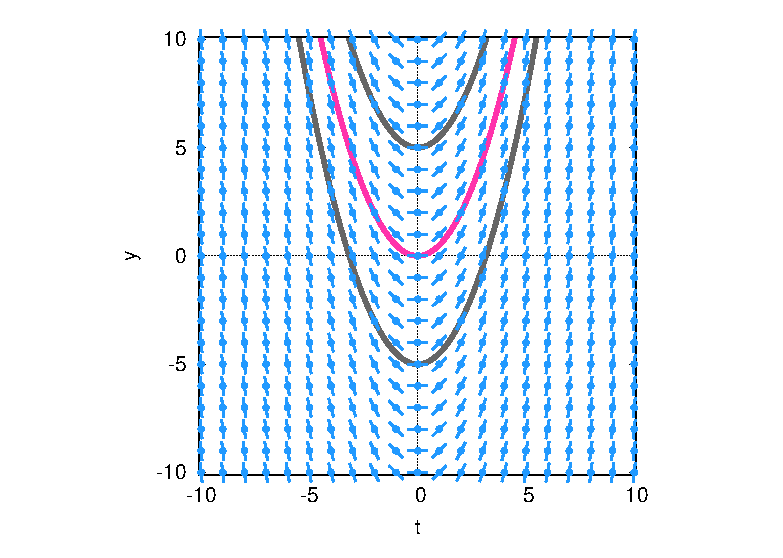
\includegraphics[width=1.0\textwidth]{fig12-3_differential_equation_t.eps}
	\end{center}
	\vspace{-5mm}
	\caption{\myfontsetting{10pt}{10pt}{$f(t,y)=t$ を図示したもの。$y=\frac{1}{2}t^2+C$ が見て取れる。}}
\end{figure}
\end{column}
\end{columns}
\end{frame}
%%%%%%%%%%%%%%%%%%%%%%%%%%%%%%%%
\begin{frame}
\frametitle{\myfontsetting{28pt}{28pt}{[図解] $f(t,y) = t^2$ の勾配場}}
\begin{columns}[t]
\begin{column}{0.48\textwidth} 
\vspace{-8mm}
\begin{itemize}
    %\setlength{\itemsep}{0.25cm}
    \item 
    \myfontsetting{12pt}{12pt}{
    $\frac{dy}{dt} = t^2$ の一般解は $y=\frac{1}{3}t^3+C$ \myfontsetting{10pt}{10pt}{($C$ は積分定数)}
    }
    \vspace{-1mm}
    \item 
    \myfontsetting{12pt}{12pt}{
    棒の傾きは $y$ 軸方向には変化せず $t$ 軸方向にのみ変化する
    }\\
    \vspace{-2mm}
    \myfontsetting{6pt}{6pt}{
    ($t=0$ で傾き0、 $t>0, t<0$ で正の傾き)
    }
    \vspace{-1mm}
    \item \myfontsetting{12pt}{12pt}{
        初期点の置き方によって縦方向にずれたどの曲線に乗るかが決まる
        \myfontsetting{10pt}{10pt}{(積分定数の不定性に対応)}
        }
\end{itemize}
\end{column}

\begin{column}{0.52\textwidth} 
\begin{figure}[h]
	\begin{center}
\vspace{-10mm}
    	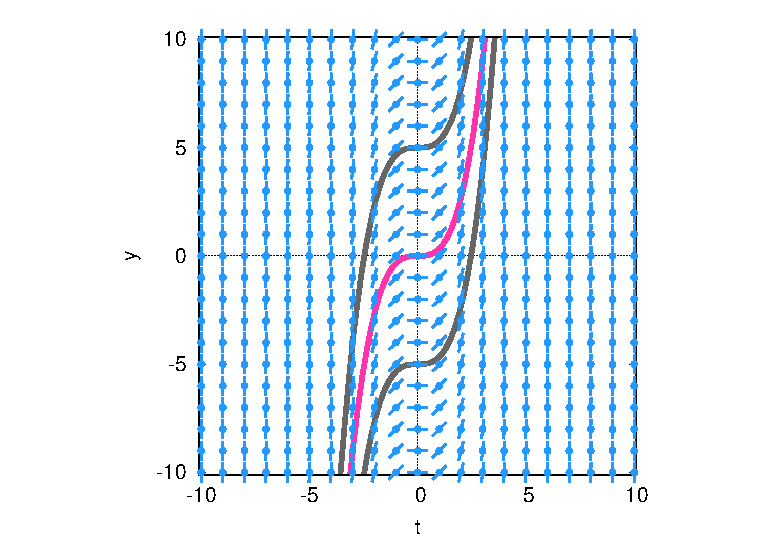
\includegraphics[width=1.0\textwidth]{fig12-4_differential_equation_tp3.eps}
	\end{center}
	\vspace{-5mm}
	\caption{\myfontsetting{10pt}{10pt}{$f(t,y)=t^2$ を図示したもの。$y=\frac{1}{3}t^3+C$ が見て取れる。}}
\end{figure}
\end{column}
\end{columns}
\end{frame}
%%%%%%%%%%%%%%%%%%%%%%%%%%%%%%%%
\begin{frame}
\frametitle{\myfontsetting{28pt}{28pt}{[図解] $f(t,y) = e^t$ の勾配場}}
\begin{columns}[t]
\begin{column}{0.48\textwidth} 
\vspace{-8mm}
\begin{itemize}
    %\setlength{\itemsep}{0.25cm}
    \item 
    \myfontsetting{12pt}{12pt}{
    $\frac{dy}{dt} = e^t$ の一般解は $y=e^t+C$ \myfontsetting{10pt}{10pt}{($C$ は積分定数)}
    }
    \vspace{-1mm}
    \item 
    \myfontsetting{12pt}{12pt}{
    棒の傾きは $y$ 軸方向には変化せず $t$ 軸方向にのみ変化する
    }\\
    \vspace{-2mm}
    \myfontsetting{6pt}{6pt}{
    ($t=0$ で傾き1)
    }
    \vspace{-1mm}
    \item \myfontsetting{12pt}{12pt}{
        初期点の置き方によって縦方向にずれたどの曲線に乗るかが決まる
        \myfontsetting{10pt}{10pt}{(積分定数の不定性に対応)}
        }
\end{itemize}
\end{column}

\begin{column}{0.52\textwidth} 
\begin{figure}[h]
	\begin{center}
\vspace{-10mm}
    	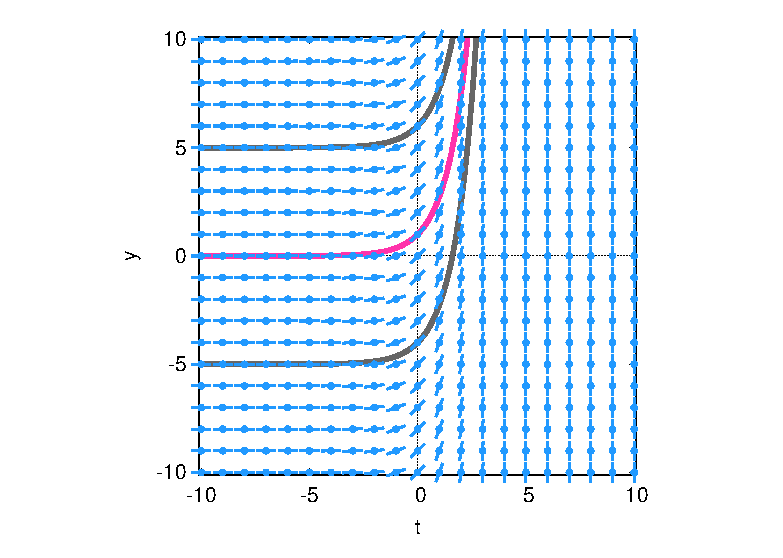
\includegraphics[width=1.0\textwidth]{fig12-5_differential_equation_exp.eps}
	\end{center}
	\vspace{-5mm}
	\caption{\myfontsetting{10pt}{10pt}{$f(t,y)=e^t$ を図示したもの。$y=e^t+C$ が見て取れる。}}
\end{figure}
\end{column}
\end{columns}
\end{frame}
%%%%%%%%%%%%%%%%%%%%%%%%%%%%%%%%
\begin{frame}
\frametitle{\myfontsetting{28pt}{28pt}{[図解] $f(t,y) = y$ の勾配場}}
\begin{columns}[t]
\begin{column}{0.48\textwidth} 
\vspace{-8mm}
\begin{itemize}
    %\setlength{\itemsep}{0.25cm}
    \item 
    \myfontsetting{12pt}{12pt}{
    $\frac{dy}{dt} = y$ の一般解は $y=\alpha e^t$ \myfontsetting{10pt}{10pt}{($\alpha$ は係数)}
    }
    \vspace{-1mm}
    \item 
    \myfontsetting{12pt}{12pt}{
    棒の傾きは $t$ 軸方向には変化せず $y$ 軸方向にのみ変化する
    }\\
    \vspace{-2mm}
    \myfontsetting{6pt}{6pt}{
    ($y=0$ で傾き0、 $y>0, y<0$ で正の傾き)
    }
    \vspace{-1mm}
    \item \myfontsetting{12pt}{12pt}{
        初期点の置き方によって縦方向にずれたどの曲線に乗るかが決まる
        \myfontsetting{10pt}{10pt}{(積分定数の不定性に対応)}
        }
\end{itemize}
\end{column}

\begin{column}{0.52\textwidth} 
\begin{figure}[h]
	\begin{center}
\vspace{-10mm}
    	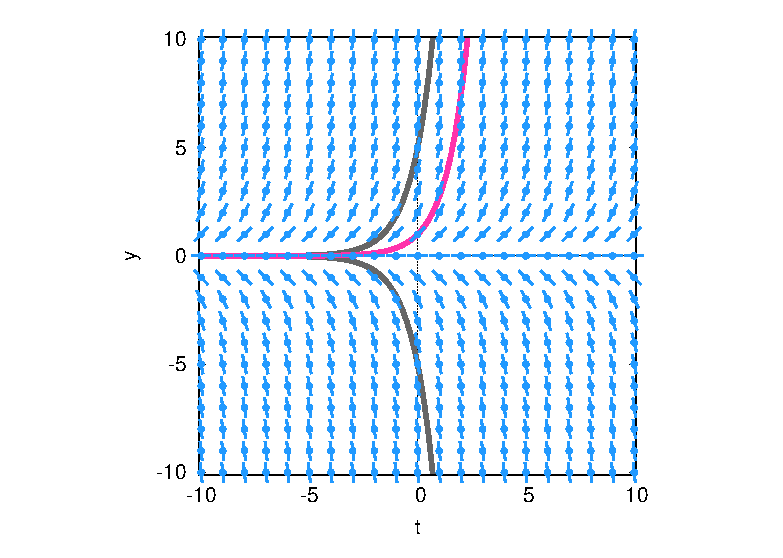
\includegraphics[width=1.0\textwidth]{fig12-6_differential_equation_y.eps}
	\end{center}
	\vspace{-5mm}
	\caption{\myfontsetting{10pt}{10pt}{$f(t,y)=y$ を図示したもの。$y=\alpha e^t$ が見て取れる。}}
\end{figure}
\end{column}
\end{columns}
\end{frame}
%%%%%%%%%%%%%%%%%%%%%%%%%%%%%%%%
\begin{frame}
\frametitle{\myfontsetting{22pt}{22pt}{[図解] $f(t,y) = y\cos(e^t + t + 1)$ の勾配場}}
\begin{columns}[t]
\begin{column}{0.48\textwidth} 
\vspace{-8mm}
\begin{itemize}
    %\setlength{\itemsep}{0.25cm}
    \item 
    \myfontsetting{12pt}{12pt}{$y=0$ が特異解。{\bf 一般解は不明}}
    \begin{itemize}
        \item \myfontsetting{10pt}{10pt}{解析解が出せなくても有限の大きさの格子上に勾配場は描ける}
    \end{itemize}
    \vspace{-1mm}
    \item \myfontsetting{12pt}{12pt}{
        出発点を決めて少しずつ $t$ 方向に歩を進めていけば $y(t)$ の形が近似として求められそう
        }
    \begin{itemize}
        \item \myfontsetting{10pt}{10pt}{常微分方程式の数値解法ではこの方針に従う}
    \end{itemize}
\end{itemize}
\end{column}

\begin{column}{0.52\textwidth} 
\begin{figure}[h]
	\begin{center}
\vspace{-10mm}
    	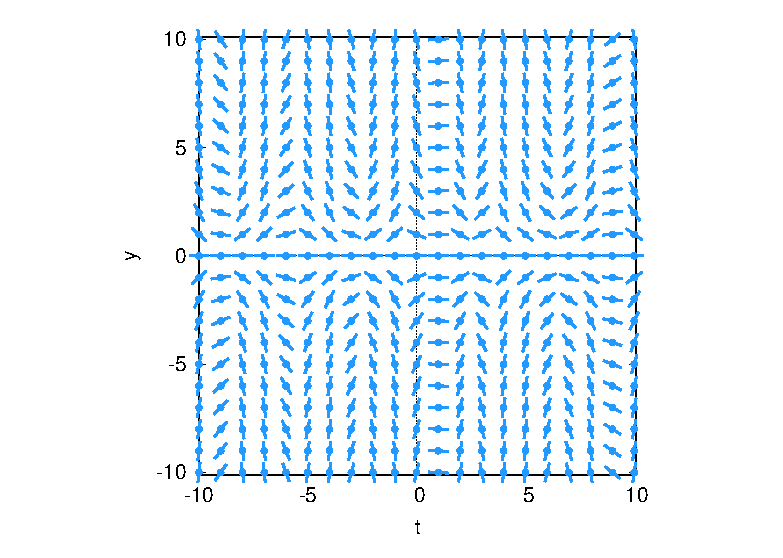
\includegraphics[width=1.0\textwidth]{fig12-7_differential_equation_difficult.eps}
	\end{center}
	\vspace{-5mm}
	\caption{\myfontsetting{10pt}{10pt}{$f(t,y) = y\cos(e^t + t + 1)$ を図示したもの。}}
\end{figure}
\end{column}
\end{columns}
\end{frame}
%%%%%%%%%%%%%%%%%%%%%%%%%%%%%%%%
\begin{frame}
\frametitle{\myfontsetting{28pt}{28pt}{常微分方程式の数値解法}}
\begin{itemize}
    \item \myfontsetting{15pt}{15pt}{\bf 問題設定}
    \begin{itemize}
        \setlength{\itemsep}{0.15cm}
        \item \myfontsetting{13pt}{13pt}{数値解法では一般解は得ることができないため、ある初期条件を決めた時に定まる $y(t)$ の近似解を求める{\bf 初期値問題} (Initial value problem) を扱う}
        \item \myfontsetting{13pt}{13pt}{初期値に対して $t$ 軸方向に小さい刻み $h$ ずつ進めて近似値を求め、その近似値を元に次の近似値を求めていく}
    \end{itemize}
    \item \myfontsetting{15pt}{15pt}{授業で扱う常微分方程式の数値解法}
    \begin{itemize}
        \setlength{\itemsep}{0.15cm}
        \item \myfontsetting{13pt}{13pt}{オイラー法、4次のルンゲ・クッタ法、蛙飛び法}
    \end{itemize}
\end{itemize}
\end{frame}
%%%%%%%%%%%%%%%%%%%%%%%%%%%%%%%%

\begin{frame}
\frametitle{\myfontsetting{28pt}{28pt}{数値積分法\myfontsetting{18pt}{18pt}{(第11回)}との違い}}
\begin{itemize}
    \setlength{\itemsep}{0.15cm}
    \item \myfontsetting{15pt}{15pt}{『$\frac{dy(t)}{dt}$ の情報を元に $y(t)$ を構成する』という意味において常微分方程式の数値解法も数値的に積分を行う手法の1種である}
    \item \myfontsetting{15pt}{15pt}{
        数値積分法 (第11回) では関数の形は予め分かっていたが常微分方程式の数値解法では積分すべき関数の形が分かっていない前提で積分を行う点が異なる}
\end{itemize}
\end{frame}
%%%%%%%%%%%%%%%%%%%%%%%%%%%%%%%%
\begin{frame}
\frametitle{[問題] X\hspace{-.1em}I\hspace{-.1em}I-A}

%%%%% START_TAG A %%%%%
%\noindent{\bf [X\hspace{-.1em}I\hspace{-.1em}I. 常微分方程式の数値解法 (1)]}%RETURN

%\noindent{\bf X\hspace{-.1em}I\hspace{-.1em}I-A.}
\myfontsetting{15pt}{18pt}{
1階の常微分方程式 $\frac{dy}{dt}=y$ について考える。\\
(1) $\frac{dy}{dt}=y$ を解析的に解くことにより一般解を求めよ。\\
(2) 上記の常微分方程式をオイラー法を用いて数値的に解く場合を考える。初期値を $(t_0,y_0)=(0,1)$、時間の刻み幅を $h=0.01$ とした時、 $y(10)$ の数値解を求めるプログラムを作成し解答せよ。また問1の答えと比べることにより相対誤差を求めよ。解答の数値は有効数字3桁で4桁目を四捨五入すること。
}\\
\myfontsetting{12pt}{12pt}{
作成したプログラムも提出すること。プログラミング言語は問わない。
}
%%%%% END_TAG A %%%%%
\end{frame}
%%%%%%%%%%%%%%%%%%%%%%%%%%%%%%%%
\begin{frame}
\frametitle{[略解] X\hspace{-.1em}I\hspace{-.1em}I-A}
%\vspace{-0.5cm}
(1) $y=e^C e^t$ ($C$ は積分定数)

\vspace{0.5cm}

(2) $\tilde{y}(10)=21000$, 相対誤差 $0.0485$
\end{frame}
%%%%%%%%%%%%%%%%%%%%%%%%%%%%%%%%

\begin{frame}
\frametitle{\myfontsetting{26pt}{26pt}{[手法解説] オイラー法} \myfontsetting{20pt}{20pt}{(Euler's method)}}
\begin{itemize}
    \setlength{\itemsep}{0.5cm}
    \item \myfontsetting{18pt}{18pt}{ある $t_i$ での値 $y(t_i)$, $f(t_i,y(t_i))$ を用いて $t_{i+1} = t_i + h$ での値を求める ({\bf 1段法}と呼ぶ)}
    \item \myfontsetting{18pt}{18pt}{$y(t+h)$ の近似方法}
    \begin{itemize}
        \setlength{\itemsep}{0.25cm}
        \item \myfontsetting{15pt}{15pt}{$y(t+h) \sim \tilde{y}(t+h) = y(t) + hf(t,y(t))$}
        \item \myfontsetting{15pt}{15pt}{テイラー展開の $h$ 1乗の項まで拾った式を使う}
    \end{itemize}
\end{itemize}
\end{frame}
%%%%%%%%%%%%%%%%%%%%%%%%%%%%%%%%
\begin{frame}
\frametitle{{\large [手法] オイラー法}}
    \begin{block}{{\bf\small オイラー法}
    \myfontsetting{13pt}{18pt}{ (Euler's method)}}
        \myfontsetting{15pt}{18pt}{
        \begin{algorithmic}[1]
            \REQUIRE $h, t_0, y_0, k$, $f(t,y)$ \hspace{2mm} \myfontsetting{10pt}{10pt}{\bf [$f(t,y)$ は関数]}
            \ENSURE $y_1,y_2,\dots, y_k$ \hspace{2mm} \myfontsetting{10pt}{10pt}{\bf [$t=t_0 + kh$ での $y$ の値の近似値]}       \FOR{$i=0,1,\dots,k-1$}
            \STATE $y_{i+1} \leftarrow y_i + f(t_i, y_i)h$
            \STATE $t_{i+1} \leftarrow t_i + h$
            \ENDFOR
        \end{algorithmic}
        }
    \end{block}
\end{frame}
%%%%%%%%%%%%%%%%%%%%%%%%%%%%%%%%
\begin{frame}
\frametitle{\myfontsetting{28pt}{28pt}{オイラー法の図解}}
\begin{columns}[t]
\begin{column}{0.48\textwidth} 
\vspace{-7mm}
\begin{itemize}
    %\setlength{\itemsep}{0.25cm}
    \item 
    \myfontsetting{13pt}{13pt}{
    初期点から(関数の傾き $\times$ 刻み幅 $h$) を継ぎ足して $y(t)$ の変化を追う方法
    }
    \item \myfontsetting{12pt}{12pt}{
    刻み幅 $h$ が小さいほど精度が良くなる
    }
    \item \myfontsetting{12pt}{12pt}{
    一般に初期点から離れるごとに精度が悪くなる
    }
\end{itemize}
\end{column}
\begin{column}{0.52\textwidth} 
\begin{figure}[h]
	\begin{center}
\vspace{-10mm}
    	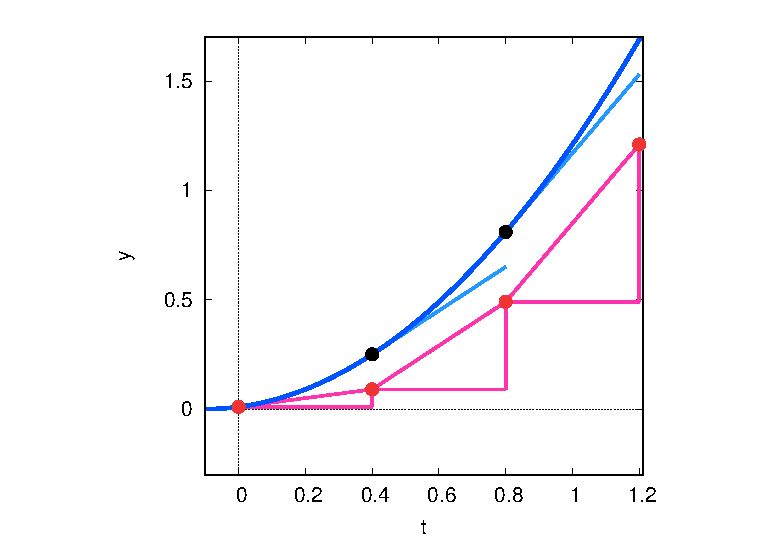
\includegraphics[width=1.0\textwidth]{fig12-8_Euler_method.eps}
	\end{center}
	\vspace{-5mm}
	\caption{\myfontsetting{8pt}{8pt}{オイラー法で3ステップ分進めて $y(t_0+3h)$ での近似値を求める %($f(t,y) = (x+0.1)^2$, $h=0.4$, $(t_0,y_0)=(0,0.01)$)
	}}
\end{figure}
\end{column}
\end{columns}
\end{frame}
%%%%%%%%%%%%%%%%%%%%%%%%%%%%%%%%
\begin{frame}
\frametitle{{\large [手法] 中点公式を使ったオイラー法}}
    \begin{block}{{\bf\small 中点公式を使ったオイラー法}\\
    \vspace{-5mm}
    \myfontsetting{13pt}{18pt}{ (Euler's method with midpoint rule)}}
        \myfontsetting{15pt}{18pt}{
        \begin{algorithmic}[1]
            \REQUIRE $h, t_0, y_0, k$, $f(t,y)$ \hspace{2mm} \myfontsetting{10pt}{10pt}{\bf [$f(t,y)$ は関数]}
            \ENSURE $y_1,y_2,\dots, y_k$ \hspace{2mm} \myfontsetting{10pt}{10pt}{\bf [$t=t_0 + kh$ での $y$ の値の近似値]}       \FOR{$i=0,1,\dots,k-1$}
            \STATE $y_{i+1} \leftarrow y_i + f\left(t_i+\frac{h}{2}, y_i+f(t_i, y_i)\frac{h}{2}\right)h$
            \STATE $t_{i+1} \leftarrow t_i + h$
            \ENDFOR
        \end{algorithmic}
        }
    \end{block}
\end{frame}
%%%%%%%%%%%%%%%%%%%%%%%%%%%%%%%%
\begin{frame}
%%%%% PASTE_START_TAG B %%%%%
%\noindent{\bf X\hspace{-.1em}I\hspace{-.1em}I-B.}
\frametitle{[問題] X\hspace{-.1em}I\hspace{-.1em}I-B}

\myfontsetting{15pt}{18pt}{
1階の常微分方程式 $\frac{dy}{dt}=y$ を4次のルンゲ・クッタ法を用いて数値的に解く場合を考える。初期値を $(t_0,y_0)=(0,1)$、時間の刻み幅を $h=0.01$ とした時、 $y(10)$ の数値解を求めるプログラムを作成し解答せよ。また $y(10)$ の真値である $22026.4657948067$ と比べることにより相対誤差を求めよ。数値解は有効数字10桁で11桁目を四捨五入し、相対誤差は有効数字3桁で4桁目を四捨五入して答えよ。
}\\
\myfontsetting{12pt}{12pt}{
作成したプログラムも提出すること。プログラミング言語は問わない。
}
%%%%% PASTE_END_TAG B %%%%%
\end{frame}

%%%%%%%%%%%%%%%%%%%%%%%%%%%%%%%%
\end{document}
